\section{experimentation}
The circuitry of a CAM can be broken down into 3 main parts. The tags, the cells and the search registers. 
The search registers are the least complex circuits in a CAM. They consist of 2 different registers, the comparand and the mask. 
The comparand is the word to search for, and the mask contains locations of bits in the word to ignore during the search.
For example, if we want to ignore the third character (or a byte) in our search, we would write mask bits [16:23] as high.
\begin{figure}
    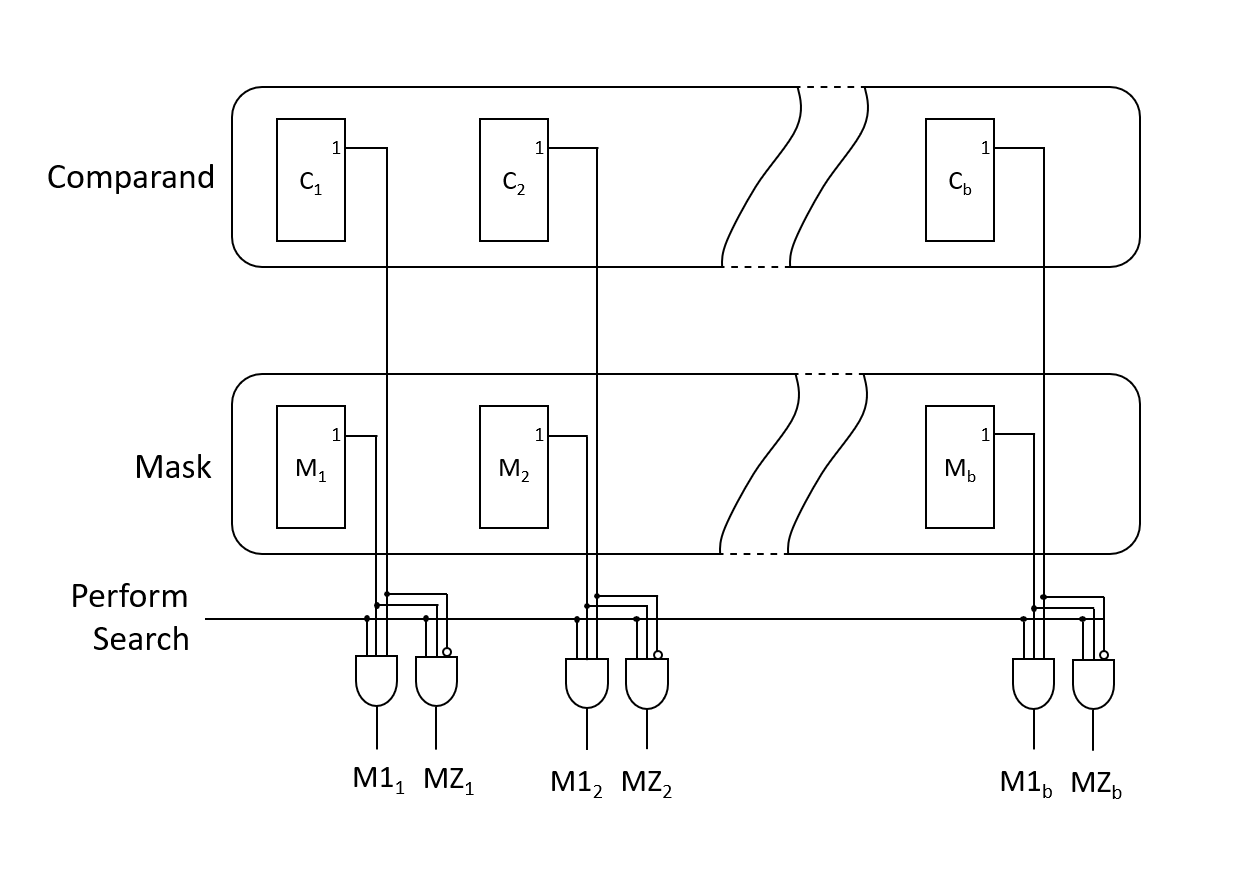
\includegraphics[width=1\columnwidth]{search_registers.png}
    \caption[Short text]{Circuitry for match lines from the search registers}
\end{figure}
\\\\
The second most complex circuitry is found in the tags, which comprises of a bits for each cell